\def\arraystretch{0.5}
\newlength\tablemathtext
\settototalheight\tablemathtext{\parbox{\linewidth}{$t=75$, $\id=446$}}
% \setlength{\tabcolsep}{1pt}
\scalebox{0.95}{
    \begin{tabular}{lccc}
        \toprule
        Time Step \& Id  & Raw Data & Segmentation & GMM fit \\ \midrule
        $t=75$, $\id=446$&
        \raisebox{\tablemathtext-\height}{
            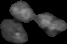
\includegraphics[width=0.18\textwidth]{images/conservation/t=75,id=446,k=3_raw.png}} &
        \raisebox{\tablemathtext-\height}{
            
\includegraphics[width=0.18\textwidth]{images/conservation/t=75,id=446,k=3_label.png}} &
        \raisebox{\tablemathtext-\height}{
            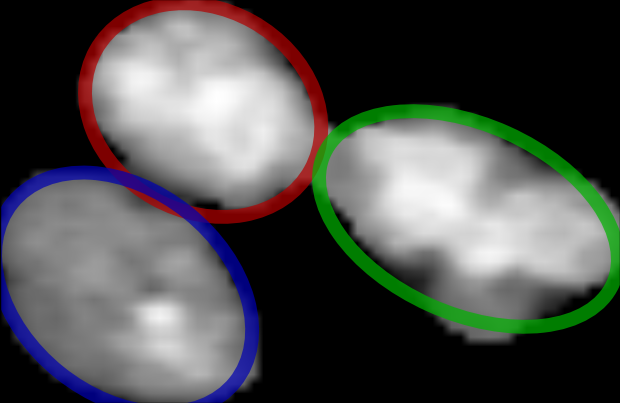
\includegraphics[width=0.18\textwidth]{images/conservation/t=75,id=446,k=3_fit.png}} \\
        &&& \\
        $t=75$, $\id=206$&
        \raisebox{\tablemathtext-\height}{
            
\includegraphics[width=0.18\textwidth]{images/conservation/t=75,id=206,k=2_raw.png}} &
        \raisebox{\tablemathtext-\height}{
            
\includegraphics[width=0.18\textwidth]{images/conservation/t=75,id=206,k=2_label.png}} &
        \raisebox{\tablemathtext-\height}{
            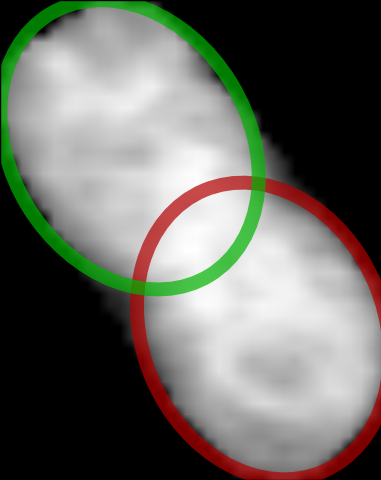
\includegraphics[width=0.18\textwidth]{images/conservation/t=75,id=206,k=2_fit.png}} \\
        &&& \\
        $t=85$, $\id=334$&
        \raisebox{\tablemathtext-\height}{
            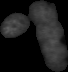
\includegraphics[width=0.18\textwidth]{images/conservation/t=85,id=334,k=4_raw.png}} &
        \raisebox{\tablemathtext-\height}{
            \hspace{-3pt}
\includegraphics[width=0.18\textwidth]{images/conservation/t=85,id=334,k=4_label.png}} &
        \raisebox{\tablemathtext-\height}{
            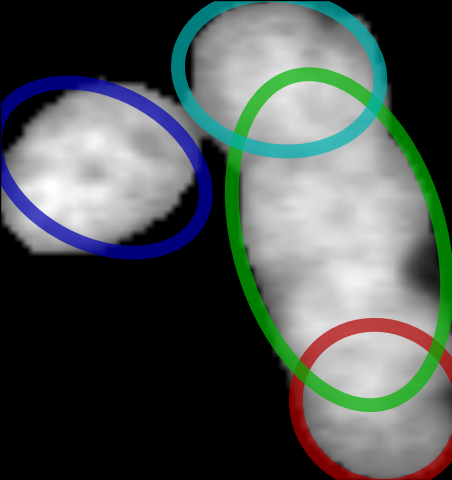
\includegraphics[width=0.18\textwidth]{images/conservation/t=85,id=334,k=4_fit.png}} \\
        \bottomrule
    \end{tabular}
}
\def\arraystretch{1.0}

% WHY THE FUCK THE NEED FOR NEGATIVE HSPACE IN LAST ROW?



%%% Local Variables: 
%%% mode: latex
%%% TeX-master: "../../main"
%%% End: 
